\section{Label Distribution}\label{sec:label_distribution}
We started by analyzing the distribution of the labels in the dataset, see Figure \ref{fig:label_dist}.
\begin{figure}[H]
    \vspace*{0.7cm}
    \centering
    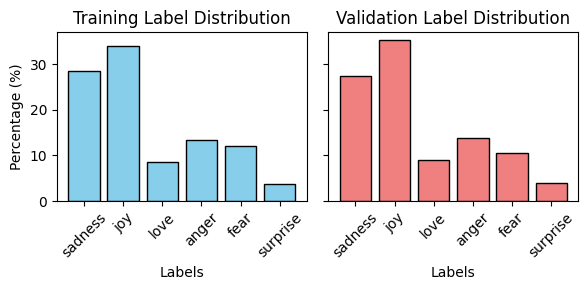
\includegraphics[width=0.5\textwidth]{figures/label_dist.png}
    \caption{Distribution of the labels in the dataset.}
    \label{fig:label_dist}
    \vspace*{0.7cm}
\end{figure}
From the figure, it is evident that the dataset is highly imbalanced, with the majority of tweets labeled as either joy or sadness. However, the validation set exhibits a roughly similar distribution of labels, suggesting that the test set is likely to follow a comparable pattern.

This imbalance in the training data is expected to impact the model's performance, particularly for less represented labels, as sentences labeled with joy are less likely to be classified correctly. This challenge must be carefully considered when evaluating the model's performance and interpreting the results.